\documentclass[11pt,a4paper]{article}

% Packages
\usepackage[margin=2.5cm]{geometry}
\usepackage{microtype}
\usepackage{graphicx}
\usepackage{tikz}
\usetikzlibrary{shapes,arrows.meta,positioning,calc,fit,backgrounds,shadows.blur,decorations.pathmorphing,decorations.pathreplacing}
\usepackage{colortbl}
\usepackage{enumitem}
\usepackage{booktabs}
\usepackage{longtable}
\usepackage{hyperref}
\usepackage{xcolor}
\usepackage{fancyhdr}
\usepackage{titlesec}
\usepackage[most]{tcolorbox}
\usepackage{multicol}
\usepackage{amsmath,amssymb}
\usepackage{multirow}
\usepackage{setspace}
\usepackage{fontawesome5}
\usepackage{listings}
\usepackage{array}
\usepackage{tabularx}

% Spacing
\setlength{\parskip}{3pt plus 1pt minus 1pt}
\setlength{\parindent}{0pt}

% Colors
\definecolor{primary}{HTML}{0B4F6C}
\definecolor{secondary}{HTML}{1A8CA0}
\definecolor{accent}{HTML}{E74C3C}
\definecolor{lightbg}{HTML}{E8F6F8}
\definecolor{defbg}{HTML}{FDF2E9}
\definecolor{greenhl}{HTML}{1E8449}
\definecolor{purplehl}{HTML}{7D3C98}
\definecolor{codebg}{HTML}{F4F6F7}
\definecolor{tealhl}{HTML}{117A65}
\definecolor{warnbg}{HTML}{FEF9E7}

% Hyperref
\hypersetup{colorlinks=true, linkcolor=primary, urlcolor=secondary, citecolor=primary}

% Code listings style
\lstset{
  backgroundcolor=\color{codebg},
  basicstyle=\ttfamily\small,
  keywordstyle=\color{primary}\bfseries,
  stringstyle=\color{greenhl},
  commentstyle=\color{gray},
  breaklines=true,
  frame=l,
  framerule=2pt,
  rulecolor=\color{secondary!40},
  xleftmargin=8pt,
  framexleftmargin=6pt,
  aboveskip=6pt,
  belowskip=6pt
}

% Header/Footer
\pagestyle{fancy}
\fancyhf{}
\fancyhead[L]{\small\textcolor{primary}{\textbf{Parallel \& Distributed Computing --- BS CS}}}
\fancyhead[R]{\small\textcolor{primary}{Midterm Exam Handout}}
\fancyfoot[C]{\small\thepage}
\fancyfoot[R]{\small\textcolor{gray!60}{April 2026}}
\renewcommand{\headrulewidth}{0.5pt}
\renewcommand{\footrulewidth}{0.3pt}

% Section formatting
\titleformat{\section}{\Large\bfseries\color{primary}}{\thesection}{0.6em}{}[\vspace{2pt}\titlerule]
\titleformat{\subsection}{\large\bfseries\color{secondary}}{\thesubsection}{0.5em}{}
\titleformat{\subsubsection}{\normalsize\bfseries\color{primary}}{\thesubsubsection}{0.5em}{}
\titlespacing*{\section}{0pt}{14pt}{8pt}
\titlespacing*{\subsection}{0pt}{10pt}{5pt}

% Custom boxes
\newtcolorbox{definitionbox}[1][]{
  enhanced, breakable,
  colback=defbg, colframe=orange!60!black,
  colbacktitle=orange!70!black, coltitle=white,
  title={\faIcon{book}~#1}, fonttitle=\bfseries,
  boxrule=0pt, leftrule=4pt, arc=2pt,
  shadow={1mm}{-1mm}{0mm}{black!15},
  top=4pt, bottom=4pt, left=8pt, right=8pt
}
\newtcolorbox{conceptbox}[1][]{
  enhanced, breakable,
  colback=lightbg, colframe=secondary,
  colbacktitle=secondary, coltitle=white,
  title={\faIcon{lightbulb}~#1}, fonttitle=\bfseries,
  boxrule=0pt, leftrule=4pt, arc=2pt,
  shadow={1mm}{-1mm}{0mm}{black!15},
  top=4pt, bottom=4pt, left=8pt, right=8pt
}
\newtcolorbox{alertbox}[1][]{
  enhanced, breakable,
  colback=red!4, colframe=accent,
  colbacktitle=accent, coltitle=white,
  title={\faIcon{exclamation-triangle}~#1}, fonttitle=\bfseries,
  boxrule=0pt, leftrule=4pt, arc=2pt,
  shadow={1mm}{-1mm}{0mm}{black!12},
  top=3pt, bottom=3pt, left=8pt, right=8pt
}
\newtcolorbox{examplebox}[1][]{
  enhanced, breakable,
  colback=green!4, colframe=greenhl,
  colbacktitle=greenhl, coltitle=white,
  title={\faIcon{code}~#1}, fonttitle=\bfseries,
  boxrule=0pt, leftrule=4pt, arc=2pt,
  shadow={1mm}{-1mm}{0mm}{black!12},
  top=3pt, bottom=3pt, left=8pt, right=8pt
}
\newtcolorbox{formulabox}[1][]{
  enhanced, breakable,
  colback=purple!4, colframe=purplehl,
  colbacktitle=purplehl, coltitle=white,
  title={\faIcon{calculator}~#1}, fonttitle=\bfseries,
  boxrule=0pt, leftrule=4pt, arc=2pt,
  shadow={1mm}{-1mm}{0mm}{black!12},
  top=4pt, bottom=4pt, left=8pt, right=8pt
}

%=======================================================================
\begin{document}

% ---- Title Page ----
\begin{center}
\vspace*{0.4cm}
{\Huge\bfseries\textcolor{primary}{Parallel \& Distributed}}\\[8pt]
{\Huge\bfseries\textcolor{primary}{Computing}}\\[16pt]
{\color{secondary}\rule{0.65\textwidth}{1.5pt}}\\[14pt]
{\Large\textsc{Midterm Exam Comprehensive Handout}}\\[8pt]
{\large\textcolor{gray!70!black}{Concepts $\bullet$ Performance $\bullet$ Synchronization $\bullet$ Communication $\bullet$ Distributed Systems}}\\[6pt]
{\normalsize\textcolor{primary!70}{BS Computer Science \quad|\quad April 2026}}
\vspace{0.3cm}
\end{center}

\begin{tcolorbox}[
  enhanced, colback=primary!6, colframe=primary,
  boxrule=1pt, arc=4pt, left=10pt, right=10pt, top=6pt, bottom=6pt
]
\textbf{\textcolor{primary}{\faIcon{clipboard-list}~Midterm Exam Coverage:}} This handout covers all foundational topics for the midterm examination including: Introduction to Parallelism, Flynn's Taxonomy, Performance Metrics (Amdahl's \& Gustafson's Laws), Parallel Algorithm Design, Process Synchronization, Inter-Process Communication, and Distributed Systems fundamentals. Study each section thoroughly, with particular attention to \textbf{formulae}, \textbf{definitions}, and \textbf{comparison tables}.
\end{tcolorbox}
\vspace{6pt}
\tableofcontents
\newpage

%=======================================================================
\section{Introduction to Parallel and Distributed Computing}
%=======================================================================

\begin{definitionbox}[Parallel Computing]
A type of computation where many calculations or processes are performed \textbf{simultaneously}. Large problems are divided into smaller ones that are solved concurrently using multiple processors.
\end{definitionbox}

\begin{definitionbox}[Distributed Computing]
A model where computation is spread across multiple \textbf{networked, autonomous computers} that communicate and coordinate by passing messages to achieve a common goal.
\end{definitionbox}

\subsection{Motivation for Parallelism}
\begin{itemize}[leftmargin=*, itemsep=3pt]
  \item \textbf{Performance:} Single-processor performance has plateaued due to physical limits (power wall, memory wall, ILP wall).
  \item \textbf{Problem Size:} Many real-world problems (weather simulation, genome analysis) are too large for a single processor.
  \item \textbf{Time Constraints:} Some tasks must be completed within strict deadlines (real-time systems, financial trading).
  \item \textbf{Cost:} Multiple commodity processors are cheaper than a single high-performance processor.
  \item \textbf{Reliability:} Distributed systems provide fault tolerance through redundancy.
\end{itemize}

\begin{center}
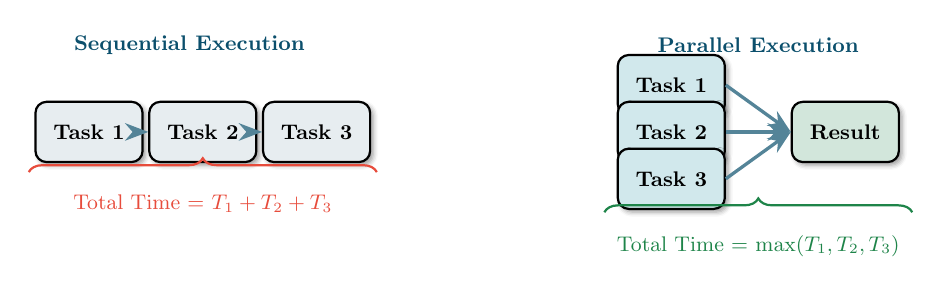
\begin{tikzpicture}[scale=0.85, transform shape,
  proc/.style={rectangle, rounded corners=4pt, draw, thick, fill=#1, minimum width=1.6cm, minimum height=0.9cm, align=center, font=\small\bfseries,
    blur shadow={shadow blur steps=4, shadow xshift=0.4mm, shadow yshift=-0.4mm}},
  arr/.style={-{Stealth}, thick, primary!70, line width=1.2pt}
]
  % Sequential label
  \node[font=\bfseries\small, primary] at (-6, 1.3) {Sequential Execution};
  \node[proc=primary!10] (t1a) at (-7.5, 0) {Task 1};
  \node[proc=primary!10] (t2a) at (-5.8, 0) {Task 2};
  \node[proc=primary!10] (t3a) at (-4.1, 0) {Task 3};
  \draw[arr] (t1a.east) -- (t2a.west);
  \draw[arr] (t2a.east) -- (t3a.west);
  \draw[decorate, decoration={brace, amplitude=5pt}, thick, accent] (-8.4,-0.6) -- (-3.2,-0.6) node[midway, below=6pt, font=\small, accent] {Total Time = $T_1 + T_2 + T_3$};

  % Parallel label
  \node[font=\bfseries\small, primary] at (2.5, 1.3) {Parallel Execution};
  \node[proc=secondary!20] (p1) at (1.2, 0.7) {Task 1};
  \node[proc=secondary!20] (p2) at (1.2, 0) {Task 2};
  \node[proc=secondary!20] (p3) at (1.2, -0.7) {Task 3};
  \node[proc=greenhl!20] (r) at (3.8, 0) {Result};
  \draw[arr] (p1.east) -- (r.west);
  \draw[arr] (p2.east) -- (r.west);
  \draw[arr] (p3.east) -- (r.west);
  \draw[decorate, decoration={brace, amplitude=5pt}, thick, greenhl] (0.2,-1.2) -- (4.8,-1.2) node[midway, below=6pt, font=\small, greenhl] {Total Time = $\max(T_1, T_2, T_3)$};
\end{tikzpicture}
\end{center}

\subsection{Parallel vs.\ Distributed Computing}

\rowcolors{2}{white}{lightbg}
\begin{longtable}{@{}p{4cm}p{5.2cm}p{5.2cm}@{}}
\toprule
\rowcolor{primary!15}
\textbf{Aspect} & \textbf{Parallel Computing} & \textbf{Distributed Computing} \\
\midrule
\endhead
\textbf{Location} & Processors at same site & Processors geographically separated \\
\textbf{Memory} & Shared or local & Each node has its own memory \\
\textbf{Communication} & Shared memory or bus & Message passing over network \\
\textbf{Synchronization} & Tight (low latency) & Loose (high latency) \\
\textbf{Failure Model} & Rare, affects whole system & Partial failures possible \\
\textbf{Goal} & Speed (performance) & Scalability \& fault tolerance \\
\textbf{Example} & Multi-core CPU, GPU & Internet, Cloud, Cluster \\
\bottomrule
\end{longtable}

%=======================================================================
\section{Flynn's Taxonomy}
%=======================================================================

\begin{conceptbox}[Flynn's Taxonomy (1966)]
A classification of computer architectures based on the number of simultaneous \textbf{instruction streams} and \textbf{data streams}. Proposed by Michael J.\ Flynn.
\end{conceptbox}

\begin{center}
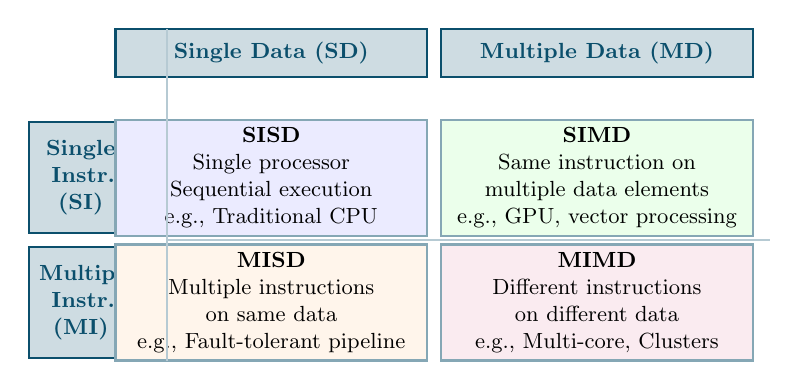
\begin{tikzpicture}[scale=0.88, transform shape,
  cell/.style={rectangle, draw=primary!50, thick, fill=#1, minimum width=4.5cm, minimum height=1.6cm, align=center, font=\small},
  hdr/.style={rectangle, draw=primary, thick, fill=primary!20, minimum width=4.5cm, minimum height=0.7cm, align=center, font=\small\bfseries\color{primary}},
  label/.style={font=\bfseries\color{primary}}
]
  % Column headers
  \node[hdr] (sd) at (0, 0) {Single Data (SD)};
  \node[hdr] (md) at (4.7, 0) {Multiple Data (MD)};
  % Row headers
  \node[hdr, minimum height=1.6cm, minimum width=1.5cm, text width=1.2cm] (si) at (-2.75, -1.8) {Single\\Instr.\\(SI)};
  \node[hdr, minimum height=1.6cm, minimum width=1.5cm, text width=1.2cm] (mi) at (-2.75, -3.6) {Multiple\\Instr.\\(MI)};
  % Cells
  \node[cell=blue!8] (sisd) at (0, -1.8) {\textbf{SISD}\\Single processor\\Sequential execution\\e.g., Traditional CPU};
  \node[cell=green!8] (simd) at (4.7, -1.8) {\textbf{SIMD}\\Same instruction on\\multiple data elements\\e.g., GPU, vector processing};
  \node[cell=orange!8] (misd) at (0, -3.6) {\textbf{MISD}\\Multiple instructions\\on same data\\e.g., Fault-tolerant pipeline};
  \node[cell=purple!8] (mimd) at (4.7, -3.6) {\textbf{MIMD}\\Different instructions\\on different data\\e.g., Multi-core, Clusters};
  % Grid lines
  \draw[primary!30, thick] (-1.5, 0.35) -- (-1.5, -4.45);
  \draw[primary!30, thick] (-1.5, -2.7) -- (7.2, -2.7);
\end{tikzpicture}
\end{center}

\begin{itemize}[leftmargin=*, itemsep=4pt]
  \item \textbf{SISD:} Classic von Neumann architecture. One processor executes one instruction at a time.
  \item \textbf{SIMD:} All processors execute the same instruction but on different data --- ideal for data-parallel tasks (image processing, neural networks). Includes SSE/AVX extensions.
  \item \textbf{MISD:} Rare in practice; mainly used in safety-critical systems (multiple processors check the same data).
  \item \textbf{MIMD:} Most common modern parallel architecture --- processors operate independently. Subdivided into:
  \begin{itemize}
    \item \textit{Shared Memory MIMD:} All processors access a global memory (SMP, multi-core).
    \item \textit{Distributed Memory MIMD:} Each processor has local memory; communicate via messages (cluster, MPI).
  \end{itemize}
\end{itemize}

%=======================================================================
\section{Types of Parallelism}
%=======================================================================

\subsection{Data Parallelism}
\begin{definitionbox}[Data Parallelism]
The same operation is applied \textbf{simultaneously to different subsets of data}. Suitable for operations that can be decomposed along data dimensions.\\[4pt]
\textbf{Example:} Multiplying each element of a 1,000,000-element array by 2 --- split the array across 4 cores, each handles 250,000 elements.
\end{definitionbox}

\subsection{Task Parallelism}
\begin{definitionbox}[Task Parallelism]
\textbf{Different tasks} (operations) are executed simultaneously on the same or different data.\\[4pt]
\textbf{Example:} While one thread downloads a file, another thread processes the already-downloaded portion.
\end{definitionbox}

\subsection{Pipeline Parallelism}
\begin{definitionbox}[Pipeline Parallelism]
A computation is divided into \textbf{stages}; while stage $i$ works on item $n$, stage $i{-}1$ already works on item $n{+}1$.\\[4pt]
\textbf{Example:} CPU instruction pipeline (Fetch $\to$ Decode $\to$ Execute $\to$ Write-back).
\end{definitionbox}

\begin{center}
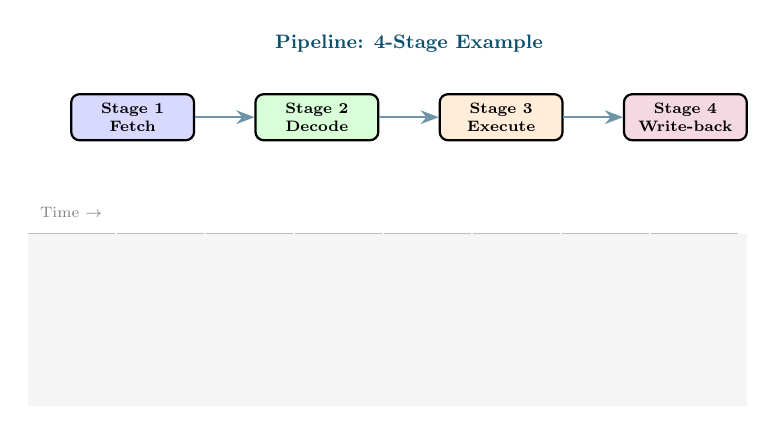
\begin{tikzpicture}[scale=0.78, transform shape,
  stage/.style={rectangle, rounded corners=3pt, draw, thick, fill=#1, minimum width=2.0cm, minimum height=0.75cm, align=center, font=\scriptsize\bfseries},
  arr/.style={-{Stealth}, thick, primary!60}
]
  \node[font=\small\bfseries, primary] at (0, 1.2) {Pipeline: 4-Stage Example};
  \node[stage=blue!15]    (s1) at (-4.5, 0) {Stage 1\\Fetch};
  \node[stage=green!15]   (s2) at (-1.5, 0) {Stage 2\\Decode};
  \node[stage=orange!15]  (s3) at (1.5, 0)  {Stage 3\\Execute};
  \node[stage=purple!15]  (s4) at (4.5, 0)  {Stage 4\\Write-back};
  \draw[arr] (s1) -- (s2);
  \draw[arr] (s2) -- (s3);
  \draw[arr] (s3) -- (s4);

  % Timeline grid
  \foreach \x/\col in {0/blue!10, 1/green!10, 2/orange!10, 3/purple!10, 4/blue!10, 5/green!10, 6/orange!10, 7/purple!10}{
    \pgfmathsetmacro{\xpos}{-5.5+\x*1.45}
    \fill[\col, opacity=0.6] (\xpos-0.7, -2.6) rectangle (\xpos+0.7, -1.9);
    \draw[black!25] (\xpos-0.7, -2.6) rectangle (\xpos+0.7, -1.9);
  }
  \foreach \y/\lbl in {0/Instr 1, 1/Instr 2, 2/Instr 3, 3/Instr 4}{
    \pgfmathsetmacro{\ypos}{-1.9-\y*0.7}
    \fill[gray!8] (-6.2, \ypos-0.7) rectangle (-6.2+11.7, \ypos);
  }
  \node[font=\scriptsize, gray] at (-5.5, -1.55) {Time $\rightarrow$};
\end{tikzpicture}
\end{center}

%=======================================================================
\section{Memory Architecture Models}
%=======================================================================

\subsection{Shared Memory Architecture}
\begin{conceptbox}[Shared Memory]
All processors access a \textbf{single global address space}. Processors communicate by reading/writing shared variables. Fast communication but limited scalability.
\end{conceptbox}

\begin{center}
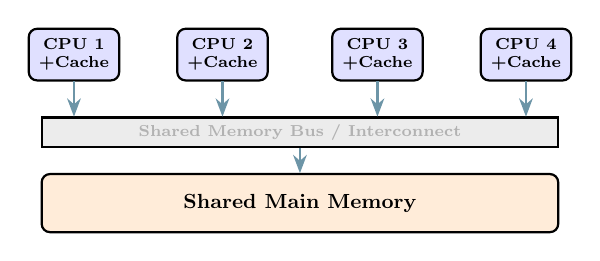
\begin{tikzpicture}[scale=0.82, transform shape,
  proc/.style={rectangle, rounded corners=3pt, draw, thick, fill=blue!12, minimum width=1.4cm, minimum height=0.8cm, align=center, font=\scriptsize\bfseries},
  mem/.style={rectangle, rounded corners=3pt, draw, thick, fill=orange!15, minimum width=8cm, minimum height=0.9cm, align=center, font=\small\bfseries},
  bus/.style={rectangle, draw, thick, fill=gray!15, minimum width=8cm, minimum height=0.45cm},
  arr/.style={-{Stealth}, thick, primary!60}
]
  \node[proc] (p1) at (-3.5, 2) {CPU 1\\+Cache};
  \node[proc] (p2) at (-1.2, 2) {CPU 2\\+Cache};
  \node[proc] (p3) at (1.2, 2)  {CPU 3\\+Cache};
  \node[proc] (p4) at (3.5, 2)  {CPU 4\\+Cache};
  \node[bus]  (bus) at (0, 0.8) {};
  \node[font=\scriptsize\bfseries, gray!60] at (0, 0.8) {Shared Memory Bus / Interconnect};
  \node[mem]  (mem) at (0, -0.3) {Shared Main Memory};
  \foreach \p in {p1, p2, p3, p4}{\draw[arr] (\p.south) -- (\p.south |- bus.north);}
  \draw[arr] (bus.south) -- (mem.north);
\end{tikzpicture}
\end{center}

\begin{itemize}[leftmargin=*, itemsep=3pt]
  \item \textbf{UMA (Uniform Memory Access):} All processors have equal memory access time. Example: SMP systems.
  \item \textbf{NUMA (Non-Uniform Memory Access):} Memory access time depends on the processor-to-memory physical location. Common in multi-socket servers.
  \item \textbf{ccNUMA:} Cache-coherent NUMA --- hardware maintains cache coherency.
\end{itemize}

\subsection{Distributed Memory Architecture}
\begin{conceptbox}[Distributed Memory]
Each processor has its \textbf{own private memory}. Processors communicate by passing messages over an interconnect network. Highly scalable, but requires explicit communication management.
\end{conceptbox}

\begin{center}
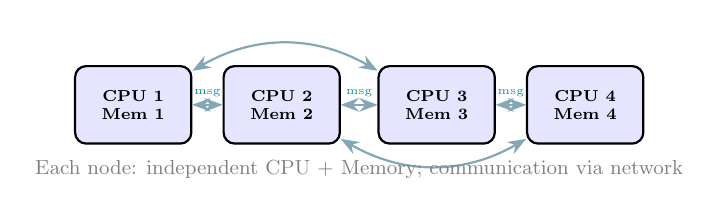
\begin{tikzpicture}[scale=0.82, transform shape,
  node_/.style={rectangle, rounded corners=4pt, draw, thick, fill=#1, minimum width=1.8cm, minimum height=1.2cm, align=center, font=\scriptsize\bfseries},
  arr/.style={Stealth-Stealth, thick, primary!50}
]
  \node[node_=blue!10]   (n1) at (-3.5, 0) {CPU 1\\Mem 1};
  \node[node_=blue!10]   (n2) at (-1.2, 0) {CPU 2\\Mem 2};
  \node[node_=blue!10]   (n3) at (1.2, 0)  {CPU 3\\Mem 3};
  \node[node_=blue!10]   (n4) at (3.5, 0)  {CPU 4\\Mem 4};
  \draw[arr] (n1) -- (n2) node[midway, above, font=\tiny, secondary] {msg};
  \draw[arr] (n2) -- (n3) node[midway, above, font=\tiny, secondary] {msg};
  \draw[arr] (n3) -- (n4) node[midway, above, font=\tiny, secondary] {msg};
  \draw[arr, bend left=30] (n1) to node[above, font=\tiny, secondary] {} (n3);
  \draw[arr, bend right=30] (n2) to node[below, font=\tiny, secondary] {} (n4);
  \node[font=\small, gray] at (0, -1.0) {Each node: independent CPU + Memory; communication via network};
\end{tikzpicture}
\end{center}

\subsection{Hybrid Architecture}
Modern supercomputers use a \textbf{hybrid model}: multiple shared-memory nodes connected via a high-speed network (e.g., InfiniBand). Example: Each compute node has a multi-core CPU (shared memory), and nodes communicate via MPI (distributed memory).

%=======================================================================
\section{Performance Metrics}
%=======================================================================

\subsection{Speedup}
\begin{formulabox}[Speedup Formula]
\[
S(p) = \frac{T_s}{T_p}
\]
\begin{itemize}[leftmargin=*, itemsep=2pt]
  \item $T_s$ = Execution time on a \textbf{single processor} (serial time)
  \item $T_p$ = Execution time on $p$ processors (parallel time)
  \item $S(p) = p$ is \textbf{linear (ideal) speedup}
  \item $S(p) > p$ is called \textbf{superlinear speedup} (rare; due to cache effects)
  \item $S(p) < p$ is typical due to overhead
\end{itemize}
\end{formulabox}

\subsection{Efficiency}
\begin{formulabox}[Efficiency Formula]
\[
E(p) = \frac{S(p)}{p} = \frac{T_s}{p \cdot T_p}
\]
\begin{itemize}[leftmargin=*, itemsep=2pt]
  \item Measures how effectively processors are being utilized.
  \item $E = 1$ (100\%): perfect efficiency (ideal)
  \item $E < 1$: processors sit idle or do redundant work
\end{itemize}
\end{formulabox}

\subsection{Amdahl's Law}
\begin{alertbox}[Amdahl's Law --- Fundamental Limit of Parallelism]
\textbf{``The speedup of a program using multiple processors is limited by the sequential fraction of the program.''}
\[
S(p) = \frac{1}{(1 - f) + \dfrac{f}{p}}
\]
\begin{itemize}[leftmargin=*, itemsep=2pt]
  \item $f$ = fraction of the program that \textbf{can} be parallelized ($0 \leq f \leq 1$)
  \item $(1-f)$ = fraction that must remain \textbf{serial}
  \item $p$ = number of processors
  \item As $p \to \infty$: $S_{\max} = \dfrac{1}{1-f}$
\end{itemize}
\textbf{Example:} If 90\% of a program is parallelizable ($f=0.9$), the maximum possible speedup is $\dfrac{1}{1-0.9} = 10\times$, no matter how many processors are used.
\end{alertbox}

\begin{center}
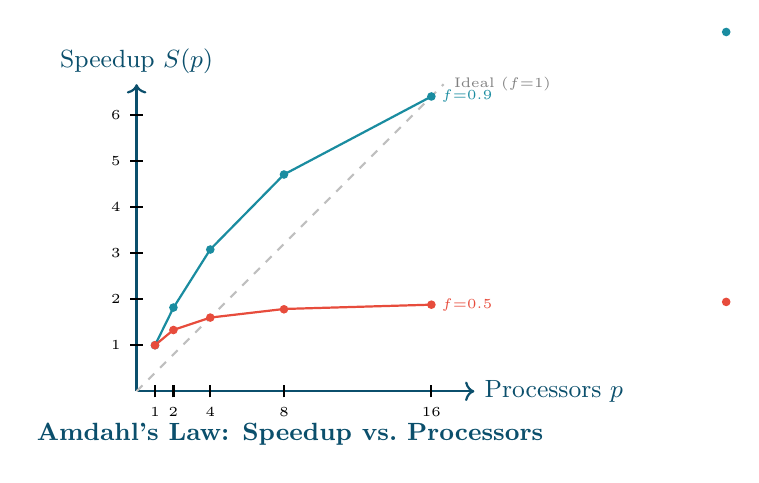
\begin{tikzpicture}[scale=0.78]
  \begin{scope}
    \draw[->, thick, primary] (0,0) -- (5.5,0) node[right, font=\small] {Processors $p$};
    \draw[->, thick, primary] (0,0) -- (0,5) node[above, font=\small] {Speedup $S(p)$};
    % Ideal
    \draw[dashed, gray!50, thick] (0,0) -- (5,5) node[right, font=\tiny, gray] {Ideal ($f{=}1$)};
    % f=0.9
    \foreach \p/\f in {1/1, 2/1.818, 4/3.077, 8/4.706, 16/6.4, 32/7.8}{
      \fill[secondary] (\p*0.3, \f*0.75) circle (2pt);
    }
    \draw[secondary, thick] (0.3,0.75)--(0.6,1.36)--(1.2,2.31)--(2.4,3.53)--(4.8,4.8) node[right, font=\tiny] {$f{=}0.9$};
    % f=0.5
    \foreach \p/\f in {1/1, 2/1.33, 4/1.6, 8/1.78, 16/1.88, 32/1.94}{
      \fill[accent] (\p*0.3, \f*0.75) circle (2pt);
    }
    \draw[accent, thick] (0.3,0.75)--(0.6,1.0)--(1.2,1.2)--(2.4,1.34)--(4.8,1.41) node[right, font=\tiny] {$f{=}0.5$};
    % Tick marks
    \foreach \x/\lbl in {0.3/1, 0.6/2, 1.2/4, 2.4/8, 4.8/16}{
      \draw[thick] (\x, -0.1) -- (\x, 0.1);
      \node[font=\tiny, below] at (\x, -0.1) {\lbl};
    }
    \foreach \y/\lbl in {0.75/1, 1.5/2, 2.25/3, 3.0/4, 3.75/5, 4.5/6}{
      \draw[thick] (-0.1, \y) -- (0.1, \y);
      \node[font=\tiny, left] at (-0.1, \y) {\lbl};
    }
    \node[font=\small\bfseries, primary] at (2.5, -0.7) {Amdahl's Law: Speedup vs.\ Processors};
  \end{scope}
\end{tikzpicture}
\end{center}

\subsection{Gustafson's Law (Scaled Speedup)}
\begin{conceptbox}[Gustafson's Law]
Unlike Amdahl's Law (which fixes problem size), Gustafson's Law assumes that as more processors are added, the \textbf{problem size scales up proportionally}.
\[
S_{\text{scaled}}(p) = p - (1-f)(p - 1) = f \cdot p + (1 - f)
\]
\begin{itemize}[leftmargin=*, itemsep=2pt]
  \item $f$ = parallel fraction of the \textbf{scaled} problem
  \item Implies that linear speedup \emph{is} achievable if problem size grows with $p$.
  \item More optimistic than Amdahl's Law for real HPC workloads.
\end{itemize}
\end{conceptbox}

\subsection{Key Performance Metrics Summary}

\rowcolors{2}{white}{lightbg}
\begin{longtable}{@{}p{4cm}p{4.5cm}p{5.2cm}@{}}
\toprule
\rowcolor{primary!15}
\textbf{Metric} & \textbf{Formula} & \textbf{Notes} \\
\midrule
\endhead
Speedup & $S = T_s / T_p$ & Ideal: $S = p$ \\
Efficiency & $E = S / p$ & Ideal: $E = 1$ (100\%) \\
Amdahl Speedup & $S = 1 / [(1-f)+f/p]$ & Limit as $p \to \infty$: $1/(1-f)$ \\
Gustafson Speedup & $S = fp + (1-f)$ & Grows linearly with $p$ \\
Scalability & $E$ stays near 1 as $p$ grows & Strong vs.\ Weak scaling \\
Communication Overhead & $T_{comm} = t_s + m/B$ & $t_s$=latency, $B$=bandwidth \\
\bottomrule
\end{longtable}

%=======================================================================
\section{Parallel Algorithm Design}
%=======================================================================

\subsection{PCAM Methodology}

\begin{conceptbox}[PCAM Design Steps (Ian Foster)]
\textbf{P}artitioning $\to$ \textbf{C}ommunication $\to$ \textbf{A}gglomeration $\to$ \textbf{M}apping
\begin{enumerate}[leftmargin=*, itemsep=3pt]
  \item \textbf{Partitioning:} Break the computation into the finest-grain tasks possible (\textit{domain decomposition} or \textit{functional decomposition}).
  \item \textbf{Communication:} Identify what data must be exchanged between tasks; determine communication patterns.
  \item \textbf{Agglomeration:} Combine fine-grain tasks into larger tasks to reduce communication overhead and improve locality.
  \item \textbf{Mapping:} Assign tasks to processors to maximize processor utilization and minimize communication cost.
\end{enumerate}
\end{conceptbox}

\subsection{Decomposition Strategies}

\begin{center}
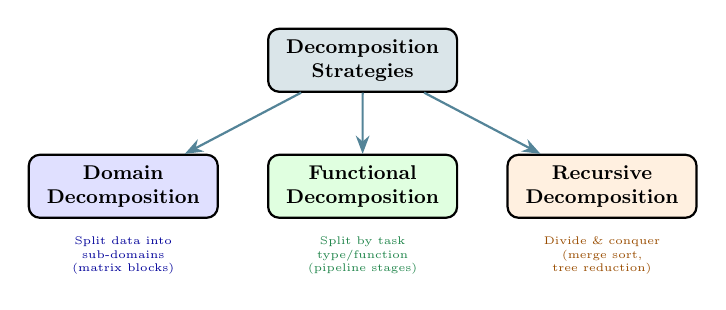
\begin{tikzpicture}[scale=0.8, transform shape,
  box/.style={rectangle, rounded corners=4pt, draw, thick, fill=#1, minimum width=3.0cm, minimum height=1.0cm, align=center, font=\small\bfseries},
  arr/.style={-{Stealth}, thick, primary!70}
]
  \node[box=primary!15] (root) at (0, 0) {Decomposition\\Strategies};
  \node[box=blue!12] (domain) at (-3.8, -2) {Domain\\Decomposition};
  \node[box=green!12] (func) at (0, -2)  {Functional\\Decomposition};
  \node[box=orange!12] (recur) at (3.8, -2)  {Recursive\\Decomposition};
  \draw[arr] (root) -- (domain);
  \draw[arr] (root) -- (func);
  \draw[arr] (root) -- (recur);
  \node[font=\tiny, align=center, blue!60!black] at (-3.8, -3.1) {Split data into\\sub-domains\\(matrix blocks)};
  \node[font=\tiny, align=center, greenhl] at (0, -3.1) {Split by task\\type/function\\(pipeline stages)};
  \node[font=\tiny, align=center, orange!60!black] at (3.8, -3.1) {Divide \& conquer\\(merge sort,\\tree reduction)};
\end{tikzpicture}
\end{center}

\subsection{Parallel Reduction}
\begin{examplebox}[Parallel Sum (Tree Reduction)]
Sum $n$ numbers using $\log_2 n$ steps instead of $n{-}1$ serial additions:
\[
\text{Step 1: } n/2 \text{ additions in parallel} \quad \to \quad \text{Step 2: } n/4 \text{ additions} \quad \to \quad \ldots \quad \to \quad 1 \text{ result}
\]
\textbf{Total steps:} $\log_2 n$ \quad \textbf{Work:} $O(n)$ \quad \textbf{Span (parallel time):} $O(\log n)$
\end{examplebox}

\subsection{Load Balancing}
\begin{itemize}[leftmargin=*, itemsep=3pt]
  \item \textbf{Static Load Balancing:} Tasks are distributed before execution begins. Simple but cannot handle variable workloads.
  \item \textbf{Dynamic Load Balancing:} Tasks are assigned at runtime based on current processor load. More flexible; requires a scheduler (work stealing, task queues).
  \item \textbf{Work Stealing:} Idle processors ``steal'' tasks from busy processors' queues. Used in Java ForkJoin, Intel TBB.
\end{itemize}

%=======================================================================
\section{Process Synchronization}
%=======================================================================

\begin{definitionbox}[Race Condition]
A situation where two or more threads/processes access \textbf{shared data concurrently}, and the final result depends on the \textbf{relative order of their execution}. This leads to \textbf{non-deterministic}, potentially incorrect behavior.
\end{definitionbox}

\begin{examplebox}[Race Condition Example]
Two threads both execute \texttt{counter = counter + 1} on a shared variable:
\begin{lstlisting}[language=C]
// Thread 1                    // Thread 2
temp1 = counter;  // reads 5   temp2 = counter;  // also reads 5
temp1 = temp1+1;  // = 6       temp2 = temp2+1;  // = 6
counter = temp1;  // writes 6  counter = temp2;  // writes 6 (lost update!)
// Expected: counter = 7,  Actual: counter = 6
\end{lstlisting}
\end{examplebox}

\subsection{Critical Section}
\begin{definitionbox}[Critical Section]
A segment of code that accesses \textbf{shared resources} and must \textbf{not be executed by more than one thread/process at a time}. A correct solution must satisfy:
\begin{enumerate}[leftmargin=*, itemsep=2pt]
  \item \textbf{Mutual Exclusion:} Only one process in the critical section at a time.
  \item \textbf{Progress:} If no process is in the critical section, one waiting process must eventually enter.
  \item \textbf{Bounded Waiting:} A process must not wait forever to enter the critical section.
\end{enumerate}
\end{definitionbox}

\subsection{Synchronization Primitives}

\subsubsection{Mutex (Mutual Exclusion Lock)}
A binary lock. A thread \textbf{acquires} (locks) the mutex before accessing shared data and \textbf{releases} (unlocks) it afterward. Only one thread can hold the mutex at a time.

\subsubsection{Semaphore}
\begin{definitionbox}[Semaphore (Dijkstra)]
An integer variable with two atomic operations:
\begin{itemize}[leftmargin=*]
  \item \textbf{P / wait / down:} Decrement the semaphore. If value $< 0$, the process blocks.
  \item \textbf{V / signal / up:} Increment the semaphore. Unblocks a waiting process.
\end{itemize}
\textbf{Binary semaphore} (0 or 1): behaves like a mutex.\\
\textbf{Counting semaphore}: controls access to a pool of $n$ resources.
\end{definitionbox}

\subsubsection{Monitor}
A higher-level synchronization construct that encapsulates shared data and its access procedures. Mutual exclusion is enforced automatically. Used in Java (\texttt{synchronized}), Python (\texttt{threading.Lock}).

\subsubsection{Barrier}
\begin{definitionbox}[Barrier Synchronization]
A synchronization point where \textbf{all processes must arrive} before any can proceed. Ensures all processes have completed a phase before the next phase begins.\\[4pt]
\textbf{Example:} In parallel matrix computation, all threads finish computing row $i$ before any starts row $i{+}1$.
\end{definitionbox}

\subsection{Deadlock}
\begin{alertbox}[Deadlock]
A situation where two or more processes are \textbf{permanently blocked}, each waiting for a resource held by another.\\[4pt]
\textbf{Four Necessary Conditions (Coffman, 1971):}
\begin{enumerate}[leftmargin=*, itemsep=2pt]
  \item \textbf{Mutual Exclusion:} Resources cannot be shared.
  \item \textbf{Hold and Wait:} A process holds at least one resource and waits for more.
  \item \textbf{No Preemption:} Resources cannot be forcibly taken from a process.
  \item \textbf{Circular Wait:} $P_1 \to P_2 \to \ldots \to P_n \to P_1$ (circular dependency chain).
\end{enumerate}
\textbf{Prevention:} Remove one of the four conditions.\\
\textbf{Avoidance:} Banker's Algorithm --- grant resources only if system stays in a safe state.\\
\textbf{Detection \& Recovery:} Allow deadlock, detect via resource-allocation graph, recover by termination or preemption.
\end{alertbox}

\subsection{Livelock and Starvation}
\begin{itemize}[leftmargin=*, itemsep=3pt]
  \item \textbf{Livelock:} Processes keep changing state in response to each other but make no progress (both keep ``politely yielding'').
  \item \textbf{Starvation:} A process is perpetually denied access to a resource because others keep getting priority (e.g., low-priority thread never runs).
\end{itemize}

%=======================================================================
\section{Inter-Process Communication (IPC)}
%=======================================================================

\subsection{Shared Memory IPC}
\begin{itemize}[leftmargin=*, itemsep=3pt]
  \item Multiple processes access a \textbf{common region of memory}.
  \item Fastest form of IPC (no kernel involvement after setup).
  \item Requires synchronization (mutexes, semaphores) to prevent race conditions.
  \item POSIX: \texttt{shm\_open()}, \texttt{mmap()}
\end{itemize}

\subsection{Message Passing}
\begin{conceptbox}[Message Passing]
Processes communicate by sending and receiving \textbf{explicit messages}. No shared memory is needed. Used in distributed systems and between processes on separate machines.
\end{conceptbox}

\begin{center}
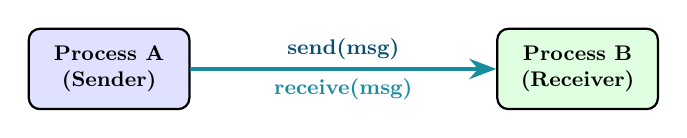
\begin{tikzpicture}[scale=0.85, transform shape,
  proc/.style={rectangle, rounded corners=4pt, draw, thick, fill=#1, minimum width=2.4cm, minimum height=1.2cm, align=center, font=\small\bfseries},
  arr/.style={-{Stealth}, thick}
]
  \node[proc=blue!12] (sender) at (-3.5, 0) {Process A\\(Sender)};
  \node[proc=green!12] (recv) at (3.5, 0) {Process B\\(Receiver)};
  \draw[arr, secondary, line width=1.5pt] (sender.east) -- (recv.west) node[midway, above, font=\small\bfseries, primary] {send(msg)} node[midway, below, font=\small\bfseries, secondary] {receive(msg)};
\end{tikzpicture}
\end{center}

\subsubsection{Blocking vs. Non-Blocking}
\rowcolors{2}{white}{lightbg}
\begin{longtable}{@{}p{3.5cm}p{5.2cm}p{5.2cm}@{}}
\toprule
\rowcolor{primary!15}
\textbf{Type} & \textbf{Blocking (Synchronous)} & \textbf{Non-Blocking (Asynchronous)} \\
\midrule
\endhead
\textbf{Send} & Sender waits until message is received & Sender continues immediately after sending \\
\textbf{Receive} & Receiver blocks until a message arrives & Receiver checks for message; continues if none \\
\textbf{Advantage} & Simple, no buffer needed & Higher concurrency \\
\textbf{Risk} & Can cause deadlock & Complex buffer management \\
\bottomrule
\end{longtable}

\subsection{MPI (Message Passing Interface) Overview}
\begin{conceptbox}[MPI Key Concepts]
The de-facto standard for message passing in HPC clusters. Key concepts:
\begin{itemize}[leftmargin=*, itemsep=3pt]
  \item \textbf{Rank:} Unique identifier (0 to $N{-}1$) for each process in a communicator.
  \item \textbf{Communicator:} A group of processes that can communicate (\texttt{MPI\_COMM\_WORLD} = all processes).
  \item \textbf{Point-to-Point:} \texttt{MPI\_Send} / \texttt{MPI\_Recv} --- one process sends to one other.
  \item \textbf{Collective Operations:} Involve all processes in a communicator.
\end{itemize}
\end{conceptbox}

\subsubsection{MPI Collective Operations}

\rowcolors{2}{white}{lightbg}
\begin{longtable}{@{}p{3.5cm}p{4cm}p{6.5cm}@{}}
\toprule
\rowcolor{primary!15}
\textbf{Operation} & \textbf{MPI Call} & \textbf{Description} \\
\midrule
\endhead
Broadcast & \texttt{MPI\_Bcast} & Root sends data to all processes \\
Scatter & \texttt{MPI\_Scatter} & Root distributes data chunks to each process \\
Gather & \texttt{MPI\_Gather} & Collects data from all processes to root \\
Reduce & \texttt{MPI\_Reduce} & Applies operation (sum, max) across all and sends to root \\
All-Reduce & \texttt{MPI\_Allreduce} & Reduce result available at all processes \\
All-to-All & \texttt{MPI\_Alltoall} & Every process sends data to every other process \\
Barrier & \texttt{MPI\_Barrier} & Synchronization point for all processes \\
\bottomrule
\end{longtable}

\subsection{Pipes and Sockets}
\begin{itemize}[leftmargin=*, itemsep=3pt]
  \item \textbf{Pipe:} Unidirectional byte stream between related processes (parent-child). Named pipes (FIFOs) work between unrelated processes.
  \item \textbf{Socket:} Bidirectional communication endpoint. Works both locally and over a network. Supports TCP (reliable) and UDP (unreliable but fast).
  \item \textbf{Message Queue:} A queue of messages managed by the OS. Processes can send/receive messages asynchronously (POSIX: \texttt{mq\_send}, \texttt{mq\_receive}).
\end{itemize}

%=======================================================================
\section{OpenMP: Shared Memory Programming}
%=======================================================================

\begin{conceptbox}[OpenMP]
An API for \textbf{shared-memory parallel programming} using compiler directives (\texttt{\#pragma omp}), library routines, and environment variables. Supports C, C++, and Fortran.
\end{conceptbox}

\begin{examplebox}[OpenMP Parallel For Loop (C)]
\begin{lstlisting}[language=C]
#include <omp.h>
int main() {
    int n = 1000; double sum = 0.0; double a[1000];
    // Parallel loop: iterations split across threads
    #pragma omp parallel for reduction(+:sum)
    for (int i = 0; i < n; i++) {
        sum += a[i];   // each thread sums its chunk
    }
    return 0;
}
\end{lstlisting}
\end{examplebox}

\subsubsection{Key OpenMP Directives}
\rowcolors{2}{white}{lightbg}
\begin{longtable}{@{}p{4.5cm}p{9cm}@{}}
\toprule
\rowcolor{primary!15}
\textbf{Directive} & \textbf{Effect} \\
\midrule
\endhead
\texttt{\#pragma omp parallel} & Creates a team of threads; each executes the block \\
\texttt{\#pragma omp for} & Distributes loop iterations across threads \\
\texttt{\#pragma omp critical} & Only one thread executes this section at a time \\
\texttt{\#pragma omp atomic} & Atomic read-modify-write for a single variable \\
\texttt{\#pragma omp barrier} & All threads wait here before proceeding \\
\texttt{reduction(op:var)} & Private copies reduced with \texttt{op} at end \\
\texttt{private(var)} & Each thread gets its own copy of \texttt{var} \\
\texttt{shared(var)} & All threads share the same \texttt{var} \\
\bottomrule
\end{longtable}

%=======================================================================
\section{Distributed Systems Fundamentals}
%=======================================================================

\begin{definitionbox}[Distributed System]
A collection of \textbf{independent computers} that appear to users as a single coherent system. The computers communicate only by \textbf{passing messages}.\\[4pt]
\textit{``A distributed system is one in which the failure of a computer you didn't even know existed can render your own computer unusable.''} --- Leslie Lamport
\end{definitionbox}

\subsection{Goals of Distributed Systems}
\begin{itemize}[leftmargin=*, itemsep=3pt]
  \item \textbf{Transparency:} Hide the fact that resources and processes are physically distributed.
  \item \textbf{Openness:} Use standard protocols and interfaces; interoperability.
  \item \textbf{Scalability:} Handle growing number of users/resources without degradation.
  \item \textbf{Fault Tolerance:} Continue operating despite partial failures.
  \item \textbf{Performance:} Achieve better throughput/latency than a single machine.
\end{itemize}

\subsubsection{Types of Transparency}
\rowcolors{2}{white}{lightbg}
\begin{longtable}{@{}p{3.8cm}p{9.5cm}@{}}
\toprule
\rowcolor{primary!15}
\textbf{Transparency Type} & \textbf{Description} \\
\midrule
\endhead
Access & Hide differences in data representation and resource access \\
Location & Users don't know the physical location of resources \\
Migration & Resources may move without affecting users \\
Replication & Multiple copies exist without users knowing \\
Concurrency & Multiple users share resources without interfering \\
Failure & Hide failure and recovery from users \\
\bottomrule
\end{longtable}

\subsection{Architectural Models}

\subsubsection{Client-Server Model}
\begin{center}
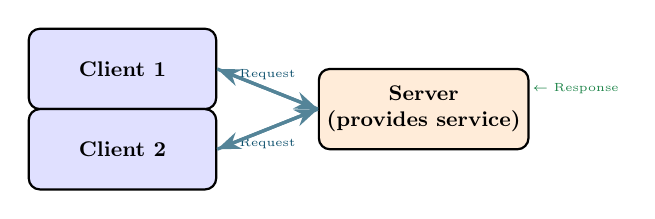
\begin{tikzpicture}[scale=0.85, transform shape,
  box/.style={rectangle, rounded corners=4pt, draw, thick, fill=#1, minimum width=2.8cm, minimum height=1.2cm, align=center, font=\small\bfseries},
  arr/.style={-{Stealth}, thick, primary!70, line width=1.2pt}
]
  \node[box=blue!12] (c1) at (-4.5, 0.6) {Client 1};
  \node[box=blue!12] (c2) at (-4.5, -0.6) {Client 2};
  \node[box=orange!15] (srv) at (0, 0) {Server\\(provides service)};
  \draw[arr] (c1.east) -- (srv.west) node[midway, above, font=\tiny, primary] {Request};
  \draw[arr] (c2.east) -- (srv.west) node[midway, below, font=\tiny, primary] {Request};
  \draw[arr] (srv.west) -- (c1.east) node[midway, above, font=\tiny, secondary] {};
  \draw[arr] (srv.west) -- (c2.east) node[midway, below, font=\tiny, secondary] {};
  \node[font=\tiny, greenhl, right] at (1.5, 0.3) {$\leftarrow$ Response};
\end{tikzpicture}
\end{center}

\begin{itemize}[leftmargin=*, itemsep=3pt]
  \item \textbf{Two-tier:} Client $\leftrightarrow$ Server (e.g., web browser + web server).
  \item \textbf{Three-tier:} Client $\leftrightarrow$ Application Server $\leftrightarrow$ Database Server.
  \item \textbf{N-tier / Microservices:} Multiple layers of services.
\end{itemize}

\subsubsection{Peer-to-Peer (P2P) Model}
All nodes are equal (peers), acting as both \textbf{client and server}. No centralized server. Examples: BitTorrent, Bitcoin, Gnutella. Provides high resilience and scalability but complicates coordination.

\subsubsection{Cloud Computing Model}
\begin{conceptbox}[Cloud Service Models]
\begin{itemize}[leftmargin=*, itemsep=3pt]
  \item \textbf{IaaS (Infrastructure as a Service):} Virtual machines, storage, networking. (e.g., AWS EC2, Azure VMs)
  \item \textbf{PaaS (Platform as a Service):} Runtime, middleware, development tools. (e.g., Google App Engine, Azure App Service)
  \item \textbf{SaaS (Software as a Service):} Ready-to-use applications. (e.g., Gmail, Microsoft 365)
\end{itemize}
\end{conceptbox}

%=======================================================================
\section{The CAP Theorem}
%=======================================================================

\begin{alertbox}[CAP Theorem (Brewer's Theorem, 2000)]
A distributed data store can guarantee \textbf{at most two} of the following three properties simultaneously:
\begin{enumerate}[leftmargin=*, itemsep=3pt]
  \item \textbf{Consistency (C):} Every read receives the \textbf{most recent write} or an error. All nodes see the same data at the same time.
  \item \textbf{Availability (A):} Every request receives a \textbf{non-error response}, even if it may not contain the most recent data.
  \item \textbf{Partition Tolerance (P):} The system continues operating despite an arbitrary number of \textbf{network partition} (message loss or failure) between nodes.
\end{enumerate}
\textbf{Implication:} In real distributed systems, network partitions \textit{will} occur, so you must choose between C and A when partitions happen.
\end{alertbox}

\begin{center}
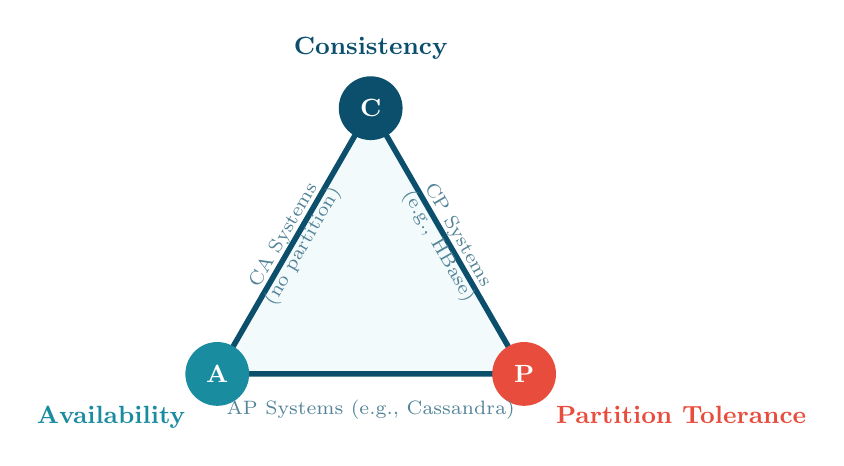
\begin{tikzpicture}[scale=0.9]
  % Triangle
  \coordinate (C) at (90:2.5);
  \coordinate (A) at (210:2.5);
  \coordinate (P) at (330:2.5);
  \fill[lightbg, opacity=0.5] (C) -- (A) -- (P) -- cycle;
  \draw[very thick, primary, line width=2pt] (C) -- (A) -- (P) -- cycle;
  % Circles at corners
  \fill[primary]   (C) circle (0.45cm); \node[white, font=\bfseries\small] at (C) {C};
  \fill[secondary] (A) circle (0.45cm); \node[white, font=\bfseries\small] at (A) {A};
  \fill[accent]    (P) circle (0.45cm); \node[white, font=\bfseries\small] at (P) {P};
  % Labels outside
  \node[font=\small\bfseries, primary, above=0.5cm]  at (C) {Consistency};
  \node[font=\small\bfseries, secondary, below left=0.4cm] at (A) {Availability};
  \node[font=\small\bfseries, accent, below right=0.4cm]  at (P) {Partition Tolerance};
  % System type labels on edges
  \node[font=\scriptsize, align=center, primary!70, rotate=60]  at ($(C)!0.5!(A)$) {CA Systems\\(no partition)};
  \node[font=\scriptsize, align=center, primary!70, rotate=-60] at ($(C)!0.5!(P)$) {CP Systems\\(e.g., HBase)};
  \node[font=\scriptsize, align=center, primary!70]             at ($(A)!0.5!(P)+(0,-0.5)$) {AP Systems (e.g., Cassandra)};
\end{tikzpicture}
\end{center}

\rowcolors{2}{white}{lightbg}
\begin{longtable}{@{}p{2.8cm}p{3.8cm}p{3.8cm}p{3.8cm}@{}}
\toprule
\rowcolor{primary!15}
\textbf{Trade-off} & \textbf{CA (no partition)} & \textbf{CP (consistent)} & \textbf{AP (available)} \\
\midrule
\endhead
Guarantees & C + A & C + P & A + P \\
Partition & Cannot tolerate & Returns error & Returns stale data \\
Examples & RDBMS (single node), 2PC & Zookeeper, HBase, MongoDB (default) & Cassandra, CouchDB, DynamoDB \\
\bottomrule
\end{longtable}

%=======================================================================
\section{Consistency Models and Replication}
%=======================================================================

\subsection{Data Replication}
\begin{itemize}[leftmargin=*, itemsep=3pt]
  \item \textbf{Purpose:} Increase availability, fault tolerance, and read performance.
  \item \textbf{Challenges:} Maintaining consistency across replicas when updates occur.
\end{itemize}

\subsection{Consistency Models}

\rowcolors{2}{white}{lightbg}
\begin{longtable}{@{}p{3.8cm}p{9.5cm}@{}}
\toprule
\rowcolor{primary!15}
\textbf{Model} & \textbf{Description} \\
\midrule
\endhead
Strong Consistency & After a write completes, all subsequent reads return that value (like a single machine). Most difficult to achieve in distributed systems. \\
Sequential Consistency & All processes see operations in the same order, but not necessarily real-time order. \\
Causal Consistency & Operations that are causally related appear in the same order to all processes. Concurrent operations may differ. \\
Eventual Consistency & Given no new updates, replicas will \textbf{eventually} converge to the same value. Used by DNS, Cassandra. \\
Read-Your-Writes & After a process writes a value, it always reads that value or a newer one in subsequent reads. \\
Monotonic Read & Successive reads by the same process never return older values. \\
\bottomrule
\end{longtable}

\subsection{Replication Strategies}
\begin{itemize}[leftmargin=*, itemsep=3pt]
  \item \textbf{Primary-Backup (Master-Slave):} One primary handles all writes; replicas follow. Simple but primary is a bottleneck.
  \item \textbf{Multi-Primary (Multi-Master):} Multiple nodes accept writes; conflict resolution required.
  \item \textbf{Quorum-Based:} A write requires acknowledgment from $W$ replicas; a read queries $R$ replicas. If $R + W > N$ (total replicas), strong consistency is guaranteed.
\end{itemize}

%=======================================================================
\section{Fault Tolerance}
%=======================================================================

\begin{definitionbox}[Fault Tolerance]
The ability of a system to \textbf{continue operating correctly} in the event of one or more failures of its components.
\end{definitionbox}

\subsection{Types of Failures}
\rowcolors{2}{white}{lightbg}
\begin{longtable}{@{}p{3.5cm}p{9.8cm}@{}}
\toprule
\rowcolor{primary!15}
\textbf{Failure Type} & \textbf{Description} \\
\midrule
\endhead
Crash Failure & A process/node stops working and does not recover (simple to handle). \\
Omission Failure & A process fails to send/receive messages it should have. \\
Timing Failure & A process responds, but outside the required time bounds. \\
Response Failure & A process responds with incorrect data (wrong value or wrong action). \\
Byzantine Failure & A process behaves arbitrarily (may send conflicting messages). Hardest to handle. \\
\bottomrule
\end{longtable}

\subsection{Fault Tolerance Techniques}
\begin{itemize}[leftmargin=*, itemsep=3pt]
  \item \textbf{Redundancy:} Replicate components so others take over on failure (hardware, software, information redundancy).
  \item \textbf{Checkpointing:} Periodically save system state so it can be restored after a failure.
  \item \textbf{Heartbeat Monitoring:} Nodes periodically send ``I'm alive'' signals; absence triggers failover.
  \item \textbf{Majority Voting:} Use odd number of replicas; accept the value agreed upon by the majority.
\end{itemize}

\subsection{Byzantine Fault Tolerance (BFT)}
\begin{conceptbox}[Byzantine Generals Problem]
$n$ processes must agree on a value, but up to $f$ of them may behave arbitrarily (send lies, different values to different nodes). Requires $n \geq 3f + 1$ processes to reach consensus despite $f$ Byzantine failures.
\end{conceptbox}

%=======================================================================
\section{Distributed Clocks and Time}
%=======================================================================

\begin{conceptbox}[The Problem with Physical Clocks]
Clocks on different machines drift and cannot be perfectly synchronized. A message sent at time $t$ on machine A may arrive at machine B when B's clock shows $t' < t$ --- violating causality.
\end{conceptbox}

\subsection{Logical Clocks}

\begin{definitionbox}[Lamport Timestamps]
Each process maintains a counter $L$. Rules:
\begin{enumerate}[leftmargin=*, itemsep=2pt]
  \item Before a process executes an event: $L \gets L + 1$.
  \item When a process sends a message: include the current $L$ in the message.
  \item When a process receives a message with timestamp $m$: $L \gets \max(L, m) + 1$.
\end{enumerate}
\textbf{Property:} If event $a$ \textit{happened-before} event $b$ (denoted $a \to b$), then $L(a) < L(b)$. But $L(a) < L(b)$ does \textbf{not} imply $a \to b$.
\end{definitionbox}

\begin{definitionbox}[Vector Clocks]
Each process $i$ maintains a vector $V_i[1..n]$. Rules:
\begin{enumerate}[leftmargin=*, itemsep=2pt]
  \item On local event: $V_i[i] \gets V_i[i] + 1$.
  \item On send: include entire vector with message.
  \item On receive from $j$ with vector $V_m$: $V_i[k] \gets \max(V_i[k], V_m[k])$ for all $k$, then $V_i[i] \gets V_i[i] + 1$.
\end{enumerate}
\textbf{Property:} $V(a) < V(b)$ if and only if $a \to b$. Captures causality precisely.
\end{definitionbox}

%=======================================================================
\section{Network Topologies for Parallel Systems}
%=======================================================================

\rowcolors{2}{white}{lightbg}
\begin{longtable}{@{}p{2.8cm}p{4.5cm}p{2.8cm}p{3.8cm}@{}}
\toprule
\rowcolor{primary!15}
\textbf{Topology} & \textbf{Description} & \textbf{Diameter} & \textbf{Bisection BW} \\
\midrule
\endhead
Bus & All nodes on single cable & 1 & 1 link \\
Ring & Each node connects to 2 neighbors & $N/2$ & 2 links \\
Mesh ($\sqrt{N}\times\sqrt{N}$) & 2D grid of nodes & $2(\sqrt{N}-1)$ & $\sqrt{N}$ links \\
Torus & Mesh with wraparound edges & $\sqrt{N}$ & $2\sqrt{N}$ links \\
Hypercube ($2^k$) & $k$-dimensional binary cube & $k = \log_2 N$ & $N/2$ links \\
Fat Tree & Multi-level tree; more BW at top & $O(\log N)$ & $N/2$ links \\
\bottomrule
\end{longtable}

\begin{center}
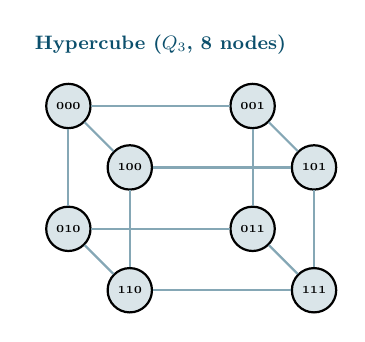
\begin{tikzpicture}[scale=0.78, transform shape,
  n/.style={circle, draw, thick, fill=primary!15, minimum size=0.55cm, font=\tiny\bfseries},
  l/.style={thick, primary!50}
]
  % Hypercube Q3
  \node[font=\small\bfseries, primary] at (0, 2.5) {Hypercube ($Q_3$, 8 nodes)};
  \node[n] (000) at (-1.5, 1.5) {000};
  \node[n] (001) at (1.5, 1.5)  {001};
  \node[n] (010) at (-1.5, -0.5) {010};
  \node[n] (011) at (1.5, -0.5) {011};
  \node[n] (100) at (-0.5, 0.5) {100};
  \node[n] (101) at (2.5, 0.5)  {101};
  \node[n] (110) at (-0.5, -1.5) {110};
  \node[n] (111) at (2.5, -1.5) {111};
  \draw[l] (000)--(001); \draw[l] (000)--(010); \draw[l] (000)--(100);
  \draw[l] (001)--(011); \draw[l] (001)--(101);
  \draw[l] (010)--(011); \draw[l] (010)--(110);
  \draw[l] (011)--(111);
  \draw[l] (100)--(101); \draw[l] (100)--(110);
  \draw[l] (101)--(111);
  \draw[l] (110)--(111);
\end{tikzpicture}
\end{center}

%=======================================================================
\section{Scalability}
%=======================================================================

\begin{definitionbox}[Scalability]
The ability of a system to handle a growing amount of work or its potential to accommodate growth.
\end{definitionbox}

\begin{itemize}[leftmargin=*, itemsep=4pt]
  \item \textbf{Strong Scaling:} The problem size is \textbf{fixed}; we add more processors to solve it faster. Limited by Amdahl's Law.
  \item \textbf{Weak Scaling:} The problem size \textbf{grows proportionally} with the number of processors; goal is to maintain constant execution time. Related to Gustafson's Law.
  \item \textbf{Horizontal Scaling (Scale Out):} Add more machines to a distributed system.
  \item \textbf{Vertical Scaling (Scale Up):} Add more resources (CPU, RAM) to existing machines.
\end{itemize}

\begin{formulabox}[Weak Scaling Efficiency]
\[
E_{\text{weak}} = \frac{T_1}{T_p}
\]
where $T_1$ = time for problem of size $n$ on 1 processor and $T_p$ = time for problem of size $n \cdot p$ on $p$ processors. Ideal: $E_{\text{weak}} = 1$.
\end{formulabox}

%=======================================================================
\section{Quick Reference: Key Formulae \& Facts}
%=======================================================================

\begin{center}
\begin{tcolorbox}[
  enhanced, colback=primary!5, colframe=primary,
  boxrule=1pt, arc=4pt, width=\textwidth,
  title={\faIcon{star}~Exam Formula \& Fact Sheet}, fonttitle=\bfseries\large,
  colbacktitle=primary, coltitle=white
]
\begin{multicols}{2}
\textbf{\textcolor{primary}{Performance Metrics:}}
\begin{itemize}[leftmargin=*, itemsep=2pt]
  \item Speedup: $S = T_s / T_p$
  \item Efficiency: $E = S/p$
  \item Amdahl's: $S = \dfrac{1}{(1-f)+f/p}$
  \item Max Speedup (Amdahl): $S_{\max} = \dfrac{1}{1-f}$
  \item Gustafson's: $S = fp + (1-f)$
\end{itemize}

\columnbreak

\textbf{\textcolor{primary}{Key Numbers to Remember:}}
\begin{itemize}[leftmargin=*, itemsep=2pt]
  \item Flynn's: SISD, SIMD, MISD, MIMD
  \item Deadlock: 4 Coffman conditions
  \item CAP: Choose 2 of 3 (C, A, P)
  \item Byzantine: need $n \geq 3f+1$ nodes
  \item Hypercube $2^k$: diameter = $k$
  \item Semaphore ops: P (wait/down), V (signal/up)
  \item Lamport: $a \to b \Rightarrow L(a) < L(b)$
\end{itemize}
\end{multicols}
\end{tcolorbox}
\end{center}

\vspace{8pt}

\begin{center}
\begin{tcolorbox}[
  enhanced, colback=orange!5, colframe=orange!70!black,
  boxrule=1pt, arc=4pt, width=\textwidth,
  title={\faIcon{tasks}~Comparison Summary}, fonttitle=\bfseries,
  colbacktitle=orange!70!black, coltitle=white
]
\rowcolors{2}{white}{orange!8}
\begin{tabular}{@{}p{4.8cm}p{4.8cm}p{4.8cm}@{}}
\toprule
\rowcolor{orange!20}
\textbf{Topic} & \textbf{Parallel} & \textbf{Distributed} \\
\midrule
Memory & Shared & Private (each node) \\
Communication & Shared variables & Message passing \\
Failure & Rare, total & Common, partial \\
Synchronization & Mutex, semaphore & Distributed protocols \\
Scalability & Limited (100s CPUs) & High (1000s nodes) \\
Example & OpenMP, CUDA & MPI, Hadoop, Cloud \\
\bottomrule
\end{tabular}
\end{tcolorbox}
\end{center}

\vspace{4pt}
\begin{center}
\textcolor{gray!60}{\small --- End of Handout --- BS CS $|$ Parallel \& Distributed Computing $|$ Midterm Exam $|$ April 2026 ---}
\end{center}

\end{document}
